\chapter{Data Analysis with \indexterm{Pandas}}
In all honesty, Python makes a bad web development language and an even worse desktop development language.\footnote{This is not a fact, the author just really hates Python for desktop and web development.} However, one of Python's biggest strengths is in scientific computing and in statistics. If you've used R before, you'll find that Python isn't that much different. In fact, both R and Python are built on the C programming language! It does use a different set of packages, but you'll find that with a little bit of statistical translation, you can do everything that you could do with a dedicated statistics programming language, such as R or SAS.\par

\section{\indexterm{Pandas} are Not Bears}
While R has much of its functionality baked right into Base-R (as a dedicated statistics language), Python requires you to load in the appropriate libraries. The hands-down most popular library is \newterm{Pandas}{Pandas}, and it's an incredibly powerful package that's appropriate for all sorts of data analysis. There are many other packages out there that are actually built on \indexterm{Pandas}, like \newterm{NumPy}{NumPy} (pronounced Num-Pie, \textit{not num-pee}), TensorFlow, Scikit-Learn, Matplotlib, Seaborn, and many others. Much of the inner workings of economics services are built using \indexterm{Pandas}, too, like Robinhood, Quandl, Morningstar, and Google Finance.\par
\funtext{\indexterm{Pandas}'s Etymology}{\indexterm{Pandas} actually stands for something: Python ANalysis for DAta. it was originally created for financial research by Wes McKinney at AQR Capital Management.}
Take your mind back to chapter 8, when we were working with a new library called \verb|csv|. Well, like \verb|csv|, \indexterm{Pandas} is also a library. In fact, we can use the same import statement as we used with \verb|csv|.
\begin{lstlisting}[style=pippython]
import pandas
\end{lstlisting}
However, when you look at most code that uses \indexterm{Pandas}, you'll notice that it's \newterm[aliased]{alias}. That means that the library name \verb|pandas| has been assigned a nickname \verb|pd| that can be used to reference library methods at any point in that script. The common \verb|pandas| alias is \verb|pd|, and we can create a library alias by using the Python keyword \verb|as|.
\begin{lstlisting}[style=pippython]
import pandas as pd
\end{lstlisting}
Now, we can access the \verb|pandas| method by using \verb|pd|. For example, instead of typing out \verb|pandas.DataFrame()|, we can just call \verb|pd.DataFrame()|.\par
\warningtext{Use pd, not something else}{Avoid creating a different alias for pandas than "pd", which has become the default alias. Using a different alias may cause confusion in readers.}
 
\boxtext{Aliases With Other Libraries}{Other libraries have well-known aliases\index{alias}, too. "numpy" is aliased "np", "scikit-learn" is aliased "sk", and "BeautifulSoup4" is aliased "bs4".}

\subsubsection*{Exercise Questions}
These exercise questions cover chapter 10.1.
\begin{Exercise}
Consider the following block of code.
\begin{lstlisting}[style=pippython]
import pandas
df = pandas.DataFrame()
\end{lstlisting}
Compare this code to the following.
\begin{lstlisting}[style=pippython]
import pandas as pd
df = pd.DataFrame()
\end{lstlisting}
What are the keywords? How are these two code chunks the same? How are they different?
\end{Exercise}
\begin{Exercise}
	\Question{What is a library alias?}
	\Question{At least three aliases were introduced to you in this section. Give some examples of aliases.}
	\Question{Why should you not use any other alias other than \verb|pd| for Pandas?}
\end{Exercise}
\begin{Exercise}
	\Question{Import a hypothetical class called \verb|Dragon| with the alias \verb|dr|.}
	\Question{Import a hypothetical class called \verb|LongLibraryNameGoesHere| with the alias \verb|longlib|.}
	\Question{Suppose there were a method inside of the \verb|Dragon| library called \verb|breath()|. How could you refer to the \verb|breath()| method if the \verb|Dragon| library were aliased with \verb|dr|?}
\end{Exercise}
\section{New Datatypes}
Learning how to use \indexterm{Pandas} means that you need to learn how to use two new datatypes: the Series\index{Pandas!series} and the new DataFrame\index{Pandas!dataframe}. These datatypes were built expressly for the purposes of data analysis while using \indexterm{Pandas}, and they build upon the initial structure of the dictionary and the list.\par
These datatypes are only available when you use \indexterm{Pandas}, so make sure you import the \indexterm{Pandas} library before trying to instantiate a new series\index{Pandas!series} or dataframe\index{Pandas!dataframe}.
\section{Series}
\newterm[Series]{Pandas!series\index{Pandas!series}} aren't used nearly as much as dataframes are in Python data analysis. Series are most akin to lists in Python, but they differ in the way that the data is stored and the methods that are available to use. However, it is possible to typecast from a Python list to a \indexterm{Pandas} series\index{Pandas!series} and vice-versa.\par
That being said, series\index{Pandas!series} are still important to cover, as they are the fundamental building blocks of dataframes, which we'll cover in the next section. Cast your mind back to when we looked at lists. A list might look like the following.
\begin{lstlisting}[style=pippython]
var1 = [56, 52, 38, 62]
\end{lstlisting}
If we look at the type of this list, we see that it's a type list.
\begin{lstlisting}[style=pippython]
type(var1)
\end{lstlisting}
\begin{lstlisting}
<class 'list'>
\end{lstlisting}
Now, let's make this Python list into a \indexterm{Pandas} series\index{Pandas!series}. Remember, a list looks like a series\index{Pandas!series}.\par
\begin{lstlisting}[style=pippython]
var1 = pd.Series(var1)
type(var1)
\end{lstlisting}
\begin{lstlisting}
<class 'pandas.core.series\index{Pandas!series}.Series'>
\end{lstlisting}
We have actually typecast the \verb|var1| object from a Python list into a \indexterm{Pandas} series\index{Pandas!series}. Observe how both series\index{Pandas!series} and lists are one-dimensional. However, what makes series\index{Pandas!series} special is how their indices are inherent and modifiable.\par
To make this list, we used the \indexterm{Pandas} \verb|Series| method. Because \verb|Series| is in the \indexterm{Pandas} class, we need to call \verb|Series| as a method on \indexterm{Pandas}, but as shown, we're using its alias \verb|pd| instead of typing out \verb|pandas|. We could just as easily type out the full class as \verb|pandas| instead of \verb|pd|.
\begin{lstlisting}[style=pippython]
var1 = pandas.Series(var1)
\end{lstlisting}
However, since the \verb|pd| moniker is so well known, we'll just use its alias.\par
In order to make a series\index{Pandas!series}, we will always use the \verb|Series| method from the \indexterm{Pandas} class. If we wanted to create an empty series\index{Pandas!series}, we would just pass nothing into the method.
\begin{lstlisting}[style=pippython]
emptySeries = pd.Series()
\end{lstlisting}
\verb|emptySeries| is of type series\index{Pandas!series}, but it has nothing in this series\index{Pandas!series}. We can also pass in a single list, as we did above.
\begin{lstlisting}[style=pippython]
var2 = pd.Series([122, 139, 185, 115])
\end{lstlisting}\par
\boxtext{Variables Versus Literals}{Notice how in \texttt{var1}, we passed in a variable with a list, while in \texttt{var2}, we passed in a list literal. As long as the datatype is correct, Python will make the series\index{Pandas!series}.}
If we tried to print the list before we typecast \verb|var1|, we would end up with something like this.
\begin{lstlisting}
[56, 52, 63, 38]
\end{lstlisting}
It prints just like any other list, complete with square brackets and commas. However, when we print our series\index{Pandas!series}, we see something a little bit different.
\begin{lstlisting}[style=pippython]
print(var1)
\end{lstlisting}
\begin{lstlisting}
0    56
1    52
2    63
3    38
dtype: int64
\end{lstlisting}
In our second column, we see the values that we typecast from our list into our series\index{Pandas!series}, but in the first column, we also see index values, starting at zero. Using this index, we can actually extract data from the series\index{Pandas!series} just as we did when we were working with lists. We will use square brackets to indicate which index we want.
\begin{lstlisting}[style=pippython]
print(var1[1])
\end{lstlisting}
\begin{lstlisting}
52
\end{lstlisting}\par
\boxtext{Indices start at zero}{Reminder: indices still start at zero, even in \indexterm{Pandas} series\index{Pandas!series}!}\par
We could also create our own indices for a series\index{Pandas!series}. Recall how we made our \verb|var1| series\index{Pandas!series}. We passed in a list only. In order to create an index, we can also pass in the argument \verb|index|, which should be of type \verb|list|.\par
\begin{lstlisting}[style=pippython]
var3 = pd.Series([3, 2, 2, 3], index = ['a', 'b', 'c', 'd'])
\end{lstlisting}
Now, if we attempt to look at \verb|var3|, we'll notice how it still has our values in the second column, but the first column has the index that we specified as a list.\par
\begin{lstlisting}
a    3
b    2
c    2
d    3
dtype: int64
\end{lstlisting}
\verb|a|, \verb|b|, \verb|c|, and \verb|d| became our index instead of the default \verb|1|, \verb|2|, \verb|3|, and \verb|4|.\par
\warningtext{Check your indices!}{Make sure that your index has the same number of elements as the data that you are putting into the array. If your indices are mismatched, you will end up with a syntax error.}
Getting data out of a series\index{Pandas!series} with an explicitly set index is similar to how we get data out of a dictionary. We still use square brackets, and we put the index that we defined. For example, if I wanted the \verb|c|'th element of the \verb|var3| series\index{Pandas!series}, I could just refer to the \verb|c|'th element as a string.\par
\begin{lstlisting}[style=pippython]
print(var3['c'])
\end{lstlisting}
\begin{lstlisting}
2
\end{lstlisting}
Because \verb|c| is of type string, we had to put our index into our square brackets inside of quotes, similar to how we need to put keys of a dictionary into quotes.\par
After learning how to change the index, you may have realized that a series\index{Pandas!series} can act like both a list \textit{or} a dictionary! If not, now you know. When we referenced our series\index{Pandas!series} without an explicit index, we could just refer to a series\index{Pandas!series} element by that index number.
\begin{lstlisting}[style=pippython]
print(var1[1])
\end{lstlisting}
\begin{lstlisting}
52
\end{lstlisting}
However, when we refer to a series\index{Pandas!series} with an explicit index, we refer to a series\index{Pandas!series} element by that index value that we set.
\begin{lstlisting}[style=pippython]
print(var3['d'])
\end{lstlisting}
\begin{lstlisting}
3
\end{lstlisting}
Let's look at a more concrete example. Consider this list which has been typecast to a series\index{Pandas!series}.
\begin{lstlisting}[style=pippython]
speeds = pd.Series([84, 93, 66, 89, 58, 59])
\end{lstlisting}
If we wanted to refer to the $n$'th element of the \verb|speeds| series\index{Pandas!series}, we would just refer to the index number as $n$.
\begin{lstlisting}[style=pippython]
print(speeds[n])
\end{lstlisting}
Now, let's consider a list which has been typecast to a series\index{Pandas!series}, but which has an explicit index.
\begin{lstlisting}[style=pippython]
agility = pd.Series([90, 90, 96, 86], index = ['Cristiano Ronaldo', 'Lionel Messi', 'Neymar', 'Luis Suarez'])
\end{lstlisting}
In order to get any of the data out of the \verb|agility| series\index{Pandas!series}, we need to know the indices or we need to just print the entire series\index{Pandas!series}.
\begin{lstlisting}[style=pippython]
print(agility)
print(agility['Neymar'])
\end{lstlisting}
\begin{lstlisting}
Cristiano Ronaldo    90
Lionel Messi         90
Neymar               96
Luis Suarez          86
dtype: int64
96
\end{lstlisting}
If we didn't want to create a dictionary-like series\index{Pandas!series} as two distinct lists (one list with the data, one list with the indices), we can actually pass in a dictionary into the \verb|Series| method and leave out the \verb|index| argument altogether. Consider the following dictionary.
\begin{lstlisting}[style=pippython]
composure = {'Cristiano Ronaldo': 86,
            'Lionel Messi': 94,
            'Neymar': 80,
            'Luis Suarez': 84}
\end{lstlisting}
If we pass this dictionary into the \verb|Series| method, \indexterm{Pandas} will typecast the dictionary into a series\index{Pandas!series} using the keys as the index and the values as the data.
\begin{lstlisting}[style=pippython]
composure = pd.Series(composure)
print(composure)
\end{lstlisting}
\begin{lstlisting}
Cristiano Ronaldo    86
Lionel Messi         94
Neymar               80
Luis Suarez          84
dtype: int64
\end{lstlisting}
Just like in a dictionary and like above, we can refer to a data value in this series\index{Pandas!series} by its index (the equivalent to a key in a dictionary, if a index were a string).
\begin{lstlisting}[style=pippython]
print(composure['Lionel Messi'])
\end{lstlisting}
\begin{lstlisting}
94
\end{lstlisting}
By now, you should have also noticed that when we print a full series\index{Pandas!series}, we also have a little line at the bottom that starts with \verb|dtype|. This tells us the type of data that is in our series\index{Pandas!series}. If all of the datatypes in a series\index{Pandas!series} are the same, the \verb|dtype| will represent that. \indexterm{Pandas} tries to store data in the simplest method possible, just like Python. So, if you pass it in an integer, it'll try to store that value as an integer, rather than a float.\par
Like a list, we can mix our datatypes between each element in a series\index{Pandas!series}. You can mix floats with integers, strings with floats, booleans with strings, and every other combination out there. However, when we mix datatypes, the \verb|dtype| that is shown somehow has to represent all of the data. Because of this mixed data, \indexterm{Pandas} will just return a datatype of "object." However, \indexterm{Pandas} will maintain the datatype in that series\index{Pandas!series} element, meaning that filling an element with a string will keep it a string, even if the \verb|dtype| of the entire series\index{Pandas!series} is listed as \verb|object|.
\begin{lstlisting}[style=pippython]
mixeddtype = pd.Series(['spinach', 48, 9.1])
print(mixeddtype)
print(type(mixeddtype))
print(mixeddtype[0], mixeddtype[1], mixeddtype[2])
print(type(mixeddtype[0]), type(mixeddtype[1]), type(mixeddtype[2]))
\end{lstlisting}
\begin{lstlisting}
0    spinach
1         48
2        9.1
dtype: object
<class 'pandas.core.series\index{Pandas!series}.Series'>
spinach 48 9.1
<class 'str'> <class 'int'> <class 'float'>
\end{lstlisting}
Observe how in the first output (where we print the entire series\index{Pandas!series}), we see that the \verb|dtype| is of type \verb|object|. This means that the elements inside of our series\index{Pandas!series} are mixed. However, the complex datatype is still a series\index{Pandas!series}. Just how we grabbed data out of our series\index{Pandas!series} before, we can do the same by referring to individual elements by index number. We can also print the datatypes of individual elements by using the \verb|type| function, where we see that all of the datatypes that we initially gave Python are maintained (string, integer, and float).\par
What if we want to add a single element to a series\index{Pandas!series}? On the surface, this seems like an easy enough topic. We've already seen an \verb|concat()| method used for lists, so it must not be too different, right? \indexterm{Pandas} actually has an \verb|concat()| method for the \verb|Series| class that will add an object of type \verb|Series| to an existing series\index{Pandas!series}. However, there is a key difference in the way that the \verb|list.concat()| works and the way the \verb|Series.concat()| method works. When we called the lists's \verb|append()| method, we simply called the method on the list, which modified the list. However, the \indexterm{Pandas} series\index{Pandas!series} \verb|concat()| method does not inherently modify that series\index{Pandas!series} like the list method does. Instead, it only returns the modified list. If we want to save this modified list, we need to pass it into a variable. The most common way to do this is by passing the return of the appended series\index{Pandas!series} back into itself, which updates the value of that variable with the appended series\index{Pandas!series}.
Consider the following list, which has three players on the Vancouver Canucks NHL team in the 2021-2022 season.\par
\begin{lstlisting}[style=pippython]
players = ["Justin Bailey", "Brock Boeser", "Madison Bowey"]
players.concat("Guillaume Briseboise")
print(players)
\end{lstlisting}
\begin{lstlisting}[style=none]
['Justin Bailey', 'Brock Boeser', 'Madison Bowey', 'Guillaume Briseboise']
\end{lstlisting}
If we try to do the same with a \indexterm{Pandas} series\index{Pandas!series}, it won't work quite the same way.
\begin{lstlisting}[style=pippython]
players = pd.Series(["Justin Bailey", "Brock Boeser", "Madison Bowey"])
players.concat("Guillaume Briseboise")
\end{lstlisting}
\begin{lstlisting}[style=none]
TypeError: cannot concatenate object of type '<class 'str'>'; only Series and DataFrame objs are valid
\end{lstlisting}
Above, we mentioned that the \verb|concat()| method on a Series will add an object of type \verb|Series| to an existing series\index{Pandas!series}, but we just tried to pass a string (\verb|"Guillaume Briseboise"|) into the \verb|concat()| method, causing a TypeError to be thrown. This is easy enough to remedy. We simply have to pass in "Guillaume Briseboise" as an element of a \indexterm{Pandas} series\index{Pandas!series}.
\begin{lstlisting}[style=pippython]
players = pd.Series(["Justin Bailey", "Brock Boeser", "Madison Bowey"])
players.concat(pd.Series(["Guillaume Briseboise"]))
\end{lstlisting}
In this case, we are passing in a \indexterm{Pandas} series\index{Pandas!series} with one element ("Guillaume Briseboise") into the \verb|concat()| method. This is especially useful if we want to pass more than one element into our series\index{Pandas!series}. For example, consider the following.
\begin{lstlisting}[style=pippython]
players = pd.Series(["Justin Bailey", "Brock Boeser", "Madison Bowey"])
players.concat(pd.Series(["Guillaume Briseboise", "Kyle Burroughs"]))
\end{lstlisting}
However, if we try to print the series\index{Pandas!series} in this state, it won't look quite right.
\begin{lstlisting}[style=pippython]
print(players)
\end{lstlisting}
\begin{lstlisting}[style=none]
0    Justin Bailey
1     Brock Boeser
2    Madison Bowey
dtype: object
\end{lstlisting}
Where are Guillaume and Kyle? Recall how we mentioned how only calling the \verb|concat()| method on the series\index{Pandas!series} object doesn't actually change the series\index{Pandas!series} object; it only returns a series\index{Pandas!series} object that has been modified. Instead, we need to put the returned series\index{Pandas!series} with the appended player names back into the \verb|players| series\index{Pandas!series}.
\begin{lstlisting}[style=pippython]
players = pd.Series(["Justin Bailey", "Brock Boeser", "Madison Bowey"])
players = players.concat(pd.Series(["Guillaume Briseboise", "Kyle Burroughs"]), ignore_index = True)
print(players)
\end{lstlisting}
\begin{lstlisting}[style=none]
0           Justin Bailey
1            Brock Boeser
2           Madison Bowey
3    Guillaume Briseboise
4          Kyle Burroughs
dtype: object
\end{lstlisting}
Recall how series\index{Pandas!series} can be indexed using a manual index. However, in this case, we never assigned a manual index when we created the series\index{Pandas!series}, hence why our \verb|players| object was assigned an auto-incrementing integer index, starting at 0. Because of this, we want \indexterm{Pandas} to ignore a possible manual index and continue to index the new row as it has indexed all of the other rows. We do this by passing in the \verb|ignore_index| argument in the \verb|concat()| method. The default is to use a null index, which we don't want, so we should specify that we want to ignore the index by setting the \verb|ignore_index| argument to \verb|True|.\par
If we don't pass in the \verb|ignore_index| argument, \indexterm{Pandas} will restart the index numbering with the appended series\index{Pandas!series}.\par
\begin{lstlisting}[style=pippython]
players = pd.Series(["Justin Bailey", "Brock Boeser", "Madison Bowey"])
players = players.concat(pd.Series(["Guillaume Briseboise", "Kyle Burroughs"]))
print(players)
\end{lstlisting}
\begin{lstlisting}[style=none]
0           Justin Bailey
1            Brock Boeser
2           Madison Bowey
0    Guillaume Briseboise
1          Kyle Burroughs
dtype: object
\end{lstlisting}

\subsubsection*{Exercise Questions}
These exercise questions cover chapter 10.3.
\begin{Exercise}
	\Question{What Python datatypes do a Pandas Series mimic?}
	\Question{What is a Pandas series?}
	\Question{What is the Pandas method to create a series?}
\end{Exercise}
\begin{Exercise}
	\Question{By default, how are Pandas series indexed?}
	\Question{If you use the default index, is a Pandas series more akin to a Python list or a Python dictionary?}
	\Question{What argument can you pass to the \verb|Series| method to set the index?}
	\Question{If you set an explicit index, is a Pandas series more akin to a Python list or a Python dictionary?}
\end{Exercise}
\begin{Exercise}
	\Question{Create a variable \verb|fruits| of type \verb|list|. Inside of the list, add the elements \verb|banana|, \verb|apple|, and \verb|orange|.}
	\Question{Typecast \verb|fruits| to a Pandas series.}
	\Question{Print the second element of the series (\verb|apple|).}
\end{Exercise}
\begin{Exercise}
	\Question{Create a variable \verb|colors| of type \verb|dict|. Inside of the dictionary, add the keys \verb|banana|, \verb|apple|, and \verb|orange| with the values \verb|yellow|, \verb|red|, and \verb|orange|, respectively.}
	\Question{Typecast \verb|colors| to a Pandas series using the keys as the index and the values as the series values.}
	\Question{Print the color of an orange.}
\end{Exercise}
\begin{Exercise}
	\Question{Create a variable \verb|bikeweights| of type \verb|pandas.Series|. Inside of the series, add the indices \verb|Canyon Ultimate CF|, \verb|Specialized Tarmac|, and \verb|Ridley Helium| with the values \verb|5.68|, \verb|6.7|, and \verb|7.57|, respectively. Do not create a dictionary to do so; instead, add your values directly to the \verb|Series| method.}
	\Question{Print the value for a Specialized Tarmac.}
	\Question{Print the value for a Canyon Ultimate CF, and append \verb|KG| to the end of the printed value.}
	\Question{Print the index and value of a Ridley Helium.}
	\Question{Add an index \verb|Trek Domane| with the value \verb|8.82| to the \verb|bikeweights| series.}
	\Question{Print the index and value of a Trek Domane, then append \verb|KG| to the end of the printed value.}
\end{Exercise}

\section{Dataframes}
Now that we've seen series\index{Pandas!series}, we can begin to explore dataframes. A dataframe\index{Pandas!dataframe} is yet another complex datatype, but it is among the most powerful of complex datatypes out there because of its flexibility and the sheer number of methods that exist to manipulate that data.\par
Most data comes to data scientists as a CSV file. Whether it's been cleaned or not, they tend to follow the same form.\par
\vspace{5mm}
\begin{tabular}{|l|l|l|l|}
\hline
id & var1 & var2 & var3 \\
\hline
1  & 56   & 122  & 3    \\
\hline
2  & 52   & 139  & 2    \\
\hline
3  & 38   & 185  & 2    \\
\hline
4  & 62   & 115  & 3    \\
\hline
\end{tabular}\par
\vspace{5mm}
The general form behind most datasets is that you have some ID to keep track of your entries and a set of variables that hold the data for each entry. This wouldn't really fit neatly into any preexisting data structure, and while we could probably write our own class to handle this data, we don't have to, since \indexterm{Pandas} comes with its own data structure that was designed to hold CSVs and other datasets: the \indexterm{Pandas} \newterm[dataframe\index{Pandas!dataframe}]{\indexterm{Pandas}!dataframe\index{Pandas!dataframe}}.\par
A dataframe\index{Pandas!dataframe} is made up of \indexterm{Pandas} series\index{Pandas!series} (hence why we covered those first). Each column of a dataframe\index{Pandas!dataframe} is composed of a single \indexterm{Pandas} series\index{Pandas!series}, and the process of putting series\index{Pandas!series} side-by-side in a certain order creates a dataframe\index{Pandas!dataframe}. However, there are two major things to note: because a dataframe\index{Pandas!dataframe} is a composite structure, you cannot edit the index of one column without altering the index of all of the columns, and the column names do not correspond to variables as they do in a pure series\index{Pandas!series}. This means that in the above series\index{Pandas!series}, we cannot simply call the \verb|var1| series\index{Pandas!series} independently of the dataframe\index{Pandas!dataframe}. We instead need to call the column as a part of the dataframe\index{Pandas!dataframe}.\par
You can think of a dataframe\index{Pandas!dataframe} as a data structure that emulates the format of a two-dimensional spreadsheet. If you are familiar with other programming languages such as C++ or C\#, then you can associate the dataframe\index{Pandas!dataframe} with a two-dimensional array.\par
\indexterm{Pandas} dataframes require you to use a certain data format in order for the data to be read and associated properly. When you import your data, you should set it up with your individual variables on row 1 and each of your trials or data entries indexed at column 1. This will allow Python to determine the datatype of an entire column. On the surface, this seems trivial, but making sure that your data is formatted correctly before you import it will mean that you'll be able to analyze it in a somewhat standard manner.\par
If your data isn't stored in the format that you required but there is some standardization to the format of the data, then consider using your already-known standard file reading and writing skills to read the file into memory, then rewrite it in the format that you require.\par
\subsection{Getting Data}
The most common operation that you'll be doing with a \indexterm{Pandas} dataframe\index{Pandas!dataframe} is retrieving data. There are a few ways to retrieve this data: we can retrieve the entire dataset as a dataframe\index{Pandas!dataframe}, typecast it to another type, or just get a subset of the data. For this section, we will cover two ways of getting data: entering it naively, and importing it from a CSV. We'll also briefly cover pickles.
\phantomsection
\subsubsection{Making a Dataframe Naively}
Let's say that you want to create a new, empty dataframe\index{Pandas!dataframe}, then put data into that empty dataframe\index{Pandas!dataframe}. You might have several lists that you want to turn into a dataframe\index{Pandas!dataframe}, or you might be reading data in from an input/output device that needs stored in a dataframe\index{Pandas!dataframe}.\par
\indexterm{Pandas} allows us to create a dataframe\index{Pandas!dataframe} by calling the \verb|.DataFrame()| method in the \indexterm{Pandas} library, and by default, it returns an empty \indexterm{Pandas} dataframe\index{Pandas!dataframe}.
\begin{lstlisting}[style=pippython]
df = pd.DataFrame()
type(df)
print(df)
\end{lstlisting}
\begin{lstlisting}[style=none]
pandas.core.frame.DataFrame
Empty DataFrame
Columns: []
Index: []
\end{lstlisting}
As you might have inferred, this is not that dissimilar for how we might have created an empty list or dictionary by calling the \verb|list()| or \verb|dict()| functions in Python. When we first create an empty dataframe\index{Pandas!dataframe}, it is assigned no size in either the row or column direction. That means that, strictly speaking, it is a zero-dimensional object.\par
The way dataframes are structured make them conducive to adding rows over columns, just like how when we make a spreadsheet in Microsoft Excel or Google Sheets, we will create the columns, then fill rows with different data. Because of this, it is much easier to define the column-wise dimension of your dataframe\index{Pandas!dataframe} than the row-wise dimension when we create the dataframe\index{Pandas!dataframe} in the first place. We can do this by passing a list type into the \verb|columns| argument of the \verb|DataFrame()| method. This will tell \indexterm{Pandas} to create columns with the names of the elements in the list that you passed in. It won't tell \indexterm{Pandas} anything about the datatypes, but at least we'll have our column-wise dimensions for our dataframe\index{Pandas!dataframe}.\par
For example, let's create a dataframe\index{Pandas!dataframe} for some ice hockey data with the column names \verb|name|, \verb|goals|, and \verb|toi|, which will stand for player name, number of goals scored, and the amount of time on the ice that they've spent, respectively. We know what our columns names will be, so we can pass these in as elements of a list into the \verb|columns| argument.\par
\begin{lstlisting}[style=pippython]
hockey = pd.DataFrame(columns = ["name", "goals", "toi"])
print(hockey)
\end{lstlisting}
\begin{lstlisting}[style=pippython]
Empty DataFrame
Columns: [name, goals, toi]
Index: []
\end{lstlisting}
\warningtext{Check your commas!}{Just a reminder to check the positions of your commas. This is just a regular list, and since we're passing in strings, our commas must fall outside of the string, otherwise Python will consider the comma to be part of the string with no demarcation between elements, which will result in a syntax error.}
Our dataframe\index{Pandas!dataframe} is still empty because there isn't any data in the row-wise dimension, but we now see that we have three columns when we print out the dataframe\index{Pandas!dataframe}.
\subsubsection{Reading a CSV}
\indexterm{Pandas} has its own method for reading in a comma-separated values, or CSV, file. Using the \indexterm{Pandas} method will allow you to put the data directly into a \indexterm{Pandas} dataframe\index{Pandas!dataframe}, rather than having to shoehorn it into a Python datatype, then typecast it to a \indexterm{Pandas} dataframe\index{Pandas!dataframe}.\par
\boxtext{Save time, use a package!}{\indexterm{Pandas} is so well universally utilized at this point that there is almost certainly a package out there for the type of data that you want to import, whether it's a R dataset (.rda or .rds), Excel worksheet (.xls or .xlsx), or OpenDocument spreadsheet (.ods). If your data is not in an easy-to-read binary file (as opposed to a plaintext file, like a CSV or TSV (tab separated values) file, consider finding a library in Pip to open the file for you and put the values into a \indexterm{Pandas} dataframe\index{Pandas!dataframe}.}
The built-in \indexterm{Pandas} method for reading a CSV file is \verb|.read_csv()|, and it returns a \indexterm{Pandas} dataframe\index{Pandas!dataframe}. The default arguments for the \verb|read_csv()| method are to read a CSV file that was created from a Microsoft Excel, Libreoffice Calc, or Google Sheets file. All three pieces of software create CSV files that adhere to some form of "typical" (although there is no standard for CSV files). For example, some CSV files may use different demarcations for strings, cells, headers, and any number of other changes.
\begin{itemize}
    \item The separator default is a comma \verb|,|, though some software separates cells using a tab (in the case of TSV files), period, or some other character.
    \item The header default is to infer whether there is one. \indexterm{Pandas} will look at the datatypes of the potential column and evaluate what datatype it is compared to the datatype of the potential header. If the datatypes match with the header, it will infer that you have no header, but if all of your header row is all strings, \indexterm{Pandas} will likely infer that you do have a header.
    \item \indexterm{Pandas} will assume that you have no indexing column and it will make its own for you.
\end{itemize}
Because these are the default arguments for the \verb|read_csv()| method, we don't need to explicitly set these arguments when we use the method. In fact, we only need to pass in one argument: the actual CSV file itself.\par
Because this is a required argument, we don't even need to specify the position of the argument in the method call. We can instead just pass in the location of the file as a string in the first position of the method call. Let's say that my file was called \verb|skaters.csv| and it was located in the current working directory. We could just run the following line to put \verb|skaters.csv| into a dataframe\index{Pandas!dataframe} called \verb|skaters|, then print the head of the \verb|skaters| dataframe\index{Pandas!dataframe}.\par
\begin{lstlisting}[style=pippython]
skaters = pd.read_csv("skaters.csv")
print(skaters.head())
\end{lstlisting}
\begin{lstlisting}[style=none]
   rank           player   playerid  ... foloss  fopct
0     1    Calen Addison  addisca01  ...      0    0.0
1     2  Andrew Agozzino  agozzan01  ...      2   33.3
2     3       Jack Ahcan  ahcanja01  ...      0    0.0
3     4    Sebastian Aho    ahose01  ...    268   52.7
4     5    Sebastian Aho    ahose02  ...      0    0.0

[5 rows x 62 columns]
\end{lstlisting}
\boxtext{Where am I?}{To find what your current working directory is, you can just run the \texttt{pwd} command in the Python shell. \texttt{pwd} stands for "print working directory."}
\boxtext{Getting Data in Subdirectories}{If your CSV file is in a subdirectory of your current working directory, you can just use slashes to indicate subdirectories. For example, if skaters.csv were a file inside of the data directory, which was inside inside of nhlskaters, which was inside of Downloads, and Downloads was my current working directory, I could just pass in "nhlskaters/data/skaters.csv". This is called a relative filepath, since you're giving the file location relative to your current working directory.}
\boxtext{Absolute Filepaths}{Sometimes, it's easier to just give the entire file string. This is called an absolute filepath. On Unix-like systems, this is easy: just preface the first directory with \texttt{/}. Your home directory is located in \texttt{/home/yourname/}. On Windows, start with \texttt{C:/} instead. Your home directory is located in \texttt{C:/Users/yourname/}.}
\subsubsection{Reading a Pickle}
Pickles are a method of storing a data in non-volatile memory that represent an entire \indexterm{Pandas} object. When a \indexterm{Pandas} object is pickled, it is stored and recalled exactly the same at the time of pickling. Consider some of the ways that we can fail to read a CSV file. If the data were created with tabs instead of commas, it would be possible to read the data incorrectly. Plus, we can't tell \indexterm{Pandas} that the first column is an index, meaning that anyone that imports the data down the line might create a new index, thus breaking your code. A pickle avoids these problems by storing the object as a whole, including indices, column names, and other metadata. This data is read when someone attempts to read the pickle, and the process of reading the pickle recreates the object exactly as it existed from whoever wrote the picklefile.\par
Essentially, writing a pickle freezes an object in time, and anyone who uses that pickle down the line will get that object exactly as it stood when it was frozen.\par
We can read pickled files using the \verb|read_pickle()| method from the \verb|Pandas| class. Because we want to get our data exactly as it was left when it was pickled, the \verb|read_pickle()| method has many fewer options compared to \verb|read_csv()|. In fact, there's really only one argument that you'll ever use when reading a pickle, and that is where the pickle is located, which is passed in as a string.\par
\begin{lstlisting}[style=pippython]
skaters = pd.read_pickle("https://github.com/pythonforscientists/data/blob/main/skaters.pkl?raw=true")
\end{lstlisting}
\subsubsection*{Exercise Questions}
These exercise questions cover chapter 10.4.1.
\begin{Exercise}
	\Question{What is a Pandas dataframe?}
	\Question{What is a Pandas dataframe made out of ?}
	\Question{If you wanted to look at the datatype of a dataframe column, what object's datatype are we actually examining?}
\end{Exercise}
\begin{Exercise}
	\Question{What is the Pandas method to create a dataframe?}
	\Question{If you call this method without passing in any arguments, what is the size of the dataframe that is created?}
	\Question{If you call this method with the \verb|columns| argument but with no values, what is the size of the dataframe that is created?}
\end{Exercise}
\begin{Exercise}
	\Question{We introduced two methods for reading two different data files. What are these methods, and what kind of files can they read?}
	\Question{If you wanted to read something other than these two data files, what would you do?}
\end{Exercise}
\begin{Exercise}
	\Question{What is the command to print your working directory?}
	\Question{What is the difference between a relative and an absolute filepath?}
\end{Exercise}
\begin{Exercise}
	\Question{Consider the method to read a CSV file. What is the Pandas method that reads a CSV file and returns a Pandas dataframe?}
	\Question{What is the separator or delimiter character that is used by default in this method?}
	\Question{Pandas dataframes need an index. If you do not specify an index in when you create a dataframe from a CSV, will Pandas create an index or will Pandas infer the index column from the data by default?}
\end{Exercise}
\begin{Exercise}
	\Question{Consider the \verb|fifa.csv| file, which is located at\\ \href{https://github.com/pythonforscientists/data/raw/main/fifa.csv}{https://github.com/pythonforscientists/data/raw/main/fifa.csv}.}
	\Question{Read the CSV file into Pandas with the default settings into a variable called \verb|fifa|.}
	\Question{Take a peek at the dataframe. What column would you use as the index?}
	\Question{Re-read the CSV file into Pandas, but this time, tell Pandas that you want to use that column as the index.}
\end{Exercise}

\subsubsection{Writing a CSV Out}
We now know how to read a CSV into our Python environment as a Pandas dataframe, but what if we want to save an existing dataframe as a CSV? Pandas also supports the writing of CSV files from dataframe objects. This makes Pandas an incredibly powerful tool for data manipulation. For example, suppose you were working with data in a different programming language, but the datafiles aren't in a format that are easy to work with. You could conceivably bring that data into Python using Pandas, manipulate it, then write a new file out that has the desired modifications.\par
Pandas provides us the \verb|to_csv()| method inside of the \verb|DataFrame| class. This means that we can call \verb|to_csv()| on any of our dataframe objects to save it as a CSV file.\par
\warningtext{Dataframes Only}{The \texttt{to\_csv()} method is a method on the \texttt{DataFrame} class in Pandas. There is no \texttt{to\_csv()} method for objects of type \texttt{Series}, so if you have a \texttt{Series} object that you want to turn into a CSV, you'll need to typecast that series into a dataframe with one column, then save that dataframe.}
The \verb|to_csv()| method takes one optional argument, which is the file to write. If no argument is passed in, Pandas will not write any file. It will, however, return the data in a CSV string.\par
Let's consider the \verb|skaters| object, which we read in as a pickle. Suppose we wanted to get the form of this data as if it were a CSV without actually writing out a CSV file. To do this, let's call the \verb|to_csv()| method on the \verb|skaters| object and put the result into a variable called \verb|skaterscsvstring|.\par
\begin{lstlisting}[style=pippython]
skaterscsvstring = skaters.to_csv()
\end{lstlisting}
If we pass in no argument, the return value of \verb|to_csv()| is the CSV-form data as a string in the variable that we chose to put the string into. That means that \verb|skatercsvstring| should now be filled with a CSV-form string. We can check this by printing the first 200 characters of the \verb|skaterscsvstring| variable.\par
\begin{lstlisting}[style=pippython]
print(skatercsvstring[:200])
\end{lstlisting}
\begin{lstlisting}[style=none]
,sid,player,playerid,age,conference,division,team,role,position,gamesplayed,cf,ca,cfpct,cfpctrel,ff,fa,ffpct,ffpctrel,toishootpct,toisavepct,pdo,offzonestartpct,defzonestartpct,toi,toieven,takeaways,g
\end{lstlisting}
Now, let's suppose that we wanted to save this object in a new file called \verb|skaters.csv| as a CSV string. Using the file handling methods that we covered in Chapter 8, we could now write the \verb|skaterscsvstring| object that we just created into a new file called \verb|skaters.csv|. However, we could also use pass in the file argument into a new \verb|to_csv()| call in Pandas.\footnote{This is generally regarded as good practice, since naively writing a file is more error-prone than using the Pandas method.}\par
So, let's pass in an argument \verb|"skaters.csv"| into the \verb|to_csv()| method.\par
\begin{lstlisting}[style=pippython]
skaters.to_csv("skaters.csv")
\end{lstlisting}
This time, we are not going to put the return of \verb|to_csv()| into any object. Rather, we passed in the argument \verb|"skaters.csv"|, so Pandas will attempt to write out a CSV file with the contents of the return value on its own. Because we specified no filepath (relative or absolute), Pandas will save \verb|skaters.csv| in our current working directory.\par
\warningtext{Permissions Pitfall}{If Python doesn't have write permissions to the directory that you are trying to save your file to, you'll end up with an \texttt{OSError} that permissions are missing. Make sure that your target directory is writable by Python. Just because \textit{you} can write a file to the directory doesn't mean that other processes on your machine can.}
\subsubsection*{Exercise Questions}
No exercise questions exist for this section.
\subsubsection{Pickling an Object}
Like writing a CSV, we may also want to write a pickle. Pickles are only readable by Pandas, but they have some advantages over reading a plaintext file. For one, picklefiles contain more than just the data. They also contain data about the data, like what the indices are, the datatypes, and the shape of the data. If we wanted to share a Pandas object with someone else who was also using Pandas, we can write a picklefile to save that object in the exact state that we left it.
\subsection{Looking at Data}
Before we can do anything with our data, we need to know what the data looks like. You could look at it in its raw form, but that doesn't really help us if we don't know that Python imported the data correctly. Luckily for us, Pandas comes with some methods that can help us get an idea of what the data looks like without necessarily giving us all of the beans.\par
\boxtext{Why not all the data?}{Why would we want to only get a little bit of the data if we wanted to get the format of data? Why not get all of it? Consider a large dataset with hundreds of thousands or even millions of rows and dozens or hundreds of columns. It would be excruciating to print that entire dataset, so having the tools to print a subset of our data is critical.}
In this section, we will cover four main methods of viewing our data: viewing the data itself, viewing the data's description, viewing a subset of the first few rows, and viewing a subset of the last few rows.\par
If we know that the size of our dataset is managable, it may make sense to just print the entire dataset. The easiest way to do this is just by using the naive \verb|print()| function in Python. When we print a Pandas dataframe, the dataframe is organized and tabulated before being printed, so it looks like a plaintext table. When we print just a dataframe, Pandas will return every single row, but it might not return every single column. If you have more than just a few columns, Pandas won't be able to print all of them, so it will abbreviate by using an ellipses to represent rows that aren't printed.\par
However, more often than not, we will be working with large datasets that don't make sense to print the entirety of. For example, let's consider the \verb|skaters| dataset that we pulled in previously. As a review, we pulled this dataset into Python as a pickle using this code.\par
\begin{lstlisting}[style=pippython]
skaters = pd.read_pickle("https://github.com/pythonforscientists/data/blob/main/skaters.pkl?raw=true")
\end{lstlisting}
Now that we've imported the data, let's look at what shape this dataframe is in. Conveniently, Pandas has an attribute called \verb|shape| that we can call on dataframe objects that will give us the shape, or dimensions, of our dataframe.\par
\warningtext{Methods versus attributes}{Cast your mind back to when we covered classes, and make sure you're not confusing your methods and your attributes. Methods are used to process data within a class, while an attribute is a feature of an object. In this case, "shape" is an attribute of the DataFrame class, not a method, so it doesn't get any parentheses.}
\begin{lstlisting}[style=pippython]
print(skaters.shape)
\end{lstlisting}
\begin{lstlisting}[style=none]
(943, 65)
\end{lstlisting}
This gave us the shape, or dimensions, of our dataframe. In this tuple, the first figure represents the number of rows, and the second figure represents the number of columns. We can see that in the \verb|skaters| dataset, we have 943 rows across 65 columns.\par
However, this doesn't actually give us what the column names are. But, guess what! There's another attribute of the DataFrame class that has the names of all of the columns, and it's named \verb|columns| (shocker, I know!).
\begin{lstlisting}[style=pippython]
print(skaters.columns)
\end{lstlisting}
\begin{lstlisting}[style=none]
Index(['sid', 'player', 'playerid', 'age', 'conference', 'division', 'team',
       'role', 'position', 'gamesplayed', 'cf', 'ca', 'cfpct', 'cfpctrel',
       'ff', 'fa', 'ffpct', 'ffpctrel', 'toishootpct', 'toisavepct', 'pdo',
       'offzonestartpct', 'defzonestartpct', 'toi', 'toieven', 'takeaways',
       'giveaways', 'expected', 'attempted', 'thrupct', 'shift', 'estoi',
       'escfpctrel', 'esgf', 'esga', 'pptoi', 'ppcfpctrel', 'ppgf', 'ppga',
       'shtoi', 'shcfpctrel', 'shgf', 'shga', 'goals', 'assists', 'points',
       'pm', 'pim', 'ps', 'evg', 'ppg', 'shg', 'gwg', 'eva', 'ppa', 'sha',
       'sog', 'shotpct', 'toi.1', 'toiavg', 'blocks', 'hits', 'fowin',
       'foloss', 'fopct'],
      dtype='object')
\end{lstlisting}
So now, we know what our columns are, but what types are they? We \textit{could} call the \verb|type()| function on an individual data cell in a column (which we'll cover how to do in a later section), or we could just look at the datatype that column is. In Pandas, we can do that by looking at the \verb|dtype| attribute of the dataframe, which will give us the datatype of all of the columns.
\begin{lstlisting}[style=pippython]
print(skaters.dtype)
\end{lstlisting}
\begin{lstlisting}[style=none]
sid             int64
player         object
playerid       object
age             int64
conference     object
               ...
blocks          int64
hits            int64
fowin           int64
foloss          int64
fopct         float64
Length: 65, dtype: object
\end{lstlisting}
Because of how many columns we have, Pandas has truncated our output to only include the first and last five columns. Since we know the names of our columns (thanks to our \verb|columns| attribute), we can also look at the datatype of an individual column.\par
\begin{lstlisting}[style=pippython]
print(skaters.dtypes["ff"])
\end{lstlisting}
\begin{lstlisting}[style=none]
dtype('int64')
\end{lstlisting}
This is how Pandas represents the data, but it might not be how Python represents the data. For example, let's look at what type the \verb|player| column is. We would expect this to be a string. It contains entries like \verb|"Michael Amadio"| and \verb|"Connor McDavid"|. However, when we call our \verb|dtypes| attribute for that column, we don't get that it's a string.\par
\begin{lstlisting}[style=pippython]
print(skaters.dtypes["players"])
\end{lstlisting}
\begin{lstlisting}[style=none]
dtype('0')
\end{lstlisting}
This is Pandas's representation of a native Python object. Pandas, frankly, doesn't care what the Python datatype is. If we want to know what \textit{kind} of object this is, we need to actually view the type of one of the rows in that column. So, let's grab the type of the first row of the \verb|player| column.
\begin{lstlisting}[style=pippython]
print(type(skaters["player"][0]))
\end{lstlisting}
\begin{lstlisting}[style=none]
str
\end{lstlisting}
We'll get into more depth on data location in the data modification section, but for your purposes now, all you need to know is that we're trying to get the type of the element from the \verb|skaters| dataframe in the \verb|"player"| column in the 0th row.
Now that we know what the datatypes are, let's actually take a look at some of this data. Remember, this is a large dataset, so we don't necessarily want to print all of it to the console. Thankfully for us, Pandas has two methods for dataframes that can give us the first $n$ rows and the last $n$ rows: \verb|head()| and \verb|tail()|.\par
\funtext{Why heads or tails?}{Pandas borrows from the Unix commands to view the first and last lines of a text file, which also use head and tail.}
We can call the \verb|head()| and \verb|tail()| methods on a dataframe object to view the first or last five rows in a dataframe, respectively.
\begin{lstlisting}[style=pippython]
print(skaters.head())
\end{lstlisting}
\begin{lstlisting}[style=none]
sid           player   playerid ... foloss fopct
0    1    Calen Addison  addisca01 ...   0   0.0
1    2  Andrew Agozzino  agozzan01 ...   2  33.3
2    3       Jack Ahcan  ahcanja01 ...   0   0.0
3    4    Sebastian Aho    ahose01 ... 268  52.7
4    5    Sebastian Aho    ahose02 ...   0   0.0

[5 rows x 65 columns]
\end{lstlisting}
\begin{lstlisting}[style=pippython]
print(skaters.tail())
\end{lstlisting}
\begin{lstlisting}[style=none]
sid           player   playerid ... foloss fopct
938  939   Mika Zibanejad  zibanmi01 ... 361  52.2
939  940    Radim Zohorna  zohorra01 ...   8  33.3
940  941        Artem Zub    zubar01 ...   0   0.0
941  942  Mats Zuccarello  zuccama01 ...  17  45.2
942  943     Jason Zucker  zuckeja01 ...  10  28.6

[5 rows x 65 columns]
\end{lstlisting}
The default value for the \verb|head()| and \verb|tail()| methods is 5, meaning that by default, calling either method will return 5 rows. However, we can also pass in a value for \verb|n| that will return \verb|n| rows. This is the only attribute that the \verb|head()| or \verb|tail()| method can take.\par
\begin{lstlisting}[style=pippython]
print(skaters.tail(10))
\end{lstlisting}
\begin{lstlisting}[style=none]
sid             player   playerid ... foloss  fopct
933  934     Nikita Zaitsev  zaitsni01 ...   0    0.0
934  935       Yegor Zamula  zamulye01 ...   0    0.0
935  936       Jakub Zboril  zborija01 ...   0    0.0
936  937      Trevor Zegras  zegratr01 ... 204   41.5
937  938  Fabian Zetterlund  zettefa01 ...   0  100.0
938  939     Mika Zibanejad  zibanmi01 ... 361   52.2
939  940      Radim Zohorna  zohorra01 ...   8   33.3
940  941          Artem Zub    zubar01 ...   0    0.0
941  942    Mats Zuccarello  zuccama01 ...  17   45.2
942  943       Jason Zucker  zuckeja01 ...  10   28.6

[10 rows x 65 columns]
\end{lstlisting}

\subsubsection*{Exercise Questions}
These exercise questions cover chapter 10.4.2.

No exercise questions exist for this section yet.

\subsection{Adding Data}
Consider the table presented in section 10.2: it looks like a table! With that view comes the advantage that we can index this table by rows and columns.\par
\boxtext{Recall}{We first saw numerical indexing when we looked at lists. Remember that in Python (and in \indexterm{Pandas}), indices start at 0, not at 1!}
We can add data in two directions: horizontally (adding a column) or vertically (adding a row), and these are done differently due to the way that dataframes are constructed. Remember, a \indexterm{Pandas} dataframe\index{Pandas!dataframe} is still a bunch of \indexterm{Pandas} series\index{Pandas!series} ordered next to each other.\par
Consider the \verb|hockey.csv| dataset. It contains 31 hockey players on the NHL Anaheim Ducks team for the 2021-2022 season. It contains the following columns: player, role, position, gamesplayed, goals, assists, fowin, foloss. For this section, we will focus on this dataset.\par
Let's start by importing this dataset. The data are located at\\ \href{https://github.com/kim3-sudo/pfs/raw/main/data/hockey.csv}{https://github.com/kim3-sudo/pfs/raw/main/data/hockey.csv} as a CSV file, so we can import it into Python as a \indexterm{Pandas} dataframe\index{Pandas!dataframe} by using the \verb|read_csv| method in \indexterm{Pandas}.\par
\boxtext{URLs or local files?}{The \texttt{read\_csv} method in \indexterm{Pandas} supports reading from a URL or from a local filepath as its argument. So, if you don't want to download the file and read it as a local file, you can also just pass in the URL of the dataset as a raw CSV file to \indexterm{Pandas} and it will pull the dataset from the Internet.}
We can read the CSV from the Internet using the \verb|read_csv| method. This CSV is formatted as most CSVs are, meaning that we don't need to pass any extra arguments into the \verb|read_csv| method: strings are in quotes, the delimiter is a comma, and there is a header.
\begin{lstlisting}[style=pippython]
hockey = pd.read_csv("https://github.com/pythonforscientists/data/raw/main/hockey.csv")
print(hockey)
\end{lstlisting}
\begin{lstlisting}[style=none]
                   player role ... fowin  foloss
0            Simon Benoit  Def ... 0       0
1             Sam Carrick  Off ... 89      90
2             Max Comtois  Off ... 14      15
3     Nicolas Deslauriers  Off ... 1       3
4          Jamie Drysdale  Def ... 0       0
5              Cam Fowler  Def ... 0       0
6            Ryan Getzlaf  Off ... 418     357
7             Derek Grant  Off ... 109     102
8   Benoit-Olivier Groulx  Off ... 38      45
9           Brendan Guhle  Def ... 0       0
10          Adam Henrique  Off ... 73      55
11              Max Jones  Off ... 1       1
12          Bryce Kindopp  Off ... 0       1
13          Jacob Larsson  Def ... 0       0
14         Vinni Lettieri  Off ... 4       1
15        Hampus Lindholm  Def ... 0       0
16        Isac Lundestrom  Off ... 267     326
17            Josh Mahura  Def ... 0       0
18            Josh Manson  Def ... 0       0
19         Mason Mctavish  Off ... 0       3
20           Sonny Milano  Off ... 0       1
21          Danny O'Regan  Off ... 8      10
22           Greg Pateryn  Def ... 0       0
23        Jacob Perreault  Off ... 0       0
24         Rickard Rakell  Off ... 28      29
25         Buddy Robinson  Off ... 0       5
26      Kevin Shattenkirk  Def ... 0       0
27      Jakob Silfverberg  Off ... 8      13
28              Sam Steel  Off ... 123     128
29             Troy Terry  Off ... 0       3
30         Brayden Tracey  Off ... 0       0

[31 rows x 8 columns]
\end{lstlisting}
When we print the data, we can see that the last player listed is Brayden Tracey, and we notice that the data are organized by the player's last name. The hockey buffs among you may have noticed one player's data is missing: Trevor Zegras.\footnote{This missing data is by design. Don't worry, Python and \indexterm{Pandas} did its job.} So, let's add a new row for Zegras's data. His data are provided below for your reference.\par
\vspace{5mm}
\begin{tabular}{|l|l|}
\hline
Column             & Value                  \\
\hline
\verb|player|      & \verb|"Trevor Zegras"| \\
\hline
\verb|role|        & \verb|"Off"|           \\
\hline
\verb|position|    & \verb|"C"|             \\
\hline
\verb|gamesplayed| & \verb|43|              \\
\hline
\verb|goals|       & \verb|12|              \\
\hline
\verb|assists|     & \verb|21|              \\
\hline
\verb|fowin|       & \verb|145|             \\
\hline
\verb|foloss|      & \verb|204|            \\
\hline
\end{tabular}\par
\vspace{5mm}
Consider how we adding data to lists. As it turns out, \indexterm{Pandas} has its own \verb|concat()| method for the \verb|DataFrame| class that will add an object of type \verb|dict| (a dictionary) to a \indexterm{Pandas} dataframe\index{Pandas!dataframe}, where the keys of the dictionary align with the column names in the dataframe\index{Pandas!dataframe}. So, let's make a dictionary with Zegras's data.
\begin{lstlisting}[style=pippython]
zegras = {
	'player': ['Trevor Zegras'],
	'role': ['Off'],
	'position': ['C'],
	'gamesplayed': [43],
	'goals': [12],
	'assists': [21],
	'fowin': [145],
	'foloss': [204]
}
\end{lstlisting}
Observe how the values in our dictionary are actually lists. This is because the \verb|concat()| method allows us to add multiple rows. If Sebastian Aho were to join the Anaheim Ducks and we wanted to add him to our dataframe, we could put his data alongside Trevor Zegras's data.\par
\begin{lstlisting}[style=pippython]
# NOT RUN
zegras = {
	'player': ['Trevor Zegras', 'Sebastian Aho'],
	'role': ['Off', 'Off'],
	'position': ['C', 'F'],
	'gamesplayed': [43, 43],
	'goals': [12, 21],
	'assists': [21, 27],
	'fowin': [145, 299],
	'foloss': [204, 268]
}
\end{lstlisting}
For the sake of demonstration, we won't create the dictionary with Sebastian Aho, only the one with Trevor Zegras. Now that the \verb|zegras| object has Trevor's data, we can use the \verb|concat()| method to concat this dictionary to the \verb|hockey| dataframe\index{Pandas!dataframe}.\cprotect\footnote{Pandas also has a method called \verb|append()| for series and dataframes that uses different syntax from \verb|concat()|. The \verb|append()| method has been deprecated, so you should avoid using it and switch to using \verb|concat()|. You may still find documentation for \verb|append()| out in the wild, but official Pandas documentation has that \verb|append()| has been deprecated in bright red. Just because it works doesn't mean that you should use it.}\par
The differences between the \verb|list.append()| and the \verb|Series.concat()| methods also exists for the \verb|DataFrame.concat()| method. Like when appending to a series\index{Pandas!series}, we need pass the return of the \verb|concat()| method back into the object.\cprotect\footnote{Assume that the \verb|zegras| dictionary object still exists here.}\par
\begin{lstlisting}[style=pippython]
hockey = pd.concat([hockey, pd.DataFrame(zegras)], ignore_index = True)
print(hockey.tail())
\end{lstlisting}
\begin{lstlisting}[style=none]
27      Jakob Silfverberg  Off ... 8      13
28              Sam Steel  Off ... 123     128
29             Troy Terry  Off ... 0       3
30         Brayden Tracey  Off ... 0       0
31          Trevor Zegras  Off ... 145     204
\end{lstlisting}
Now that we put the return of the \verb|concat()| method into the \verb|hockey| object, \verb|hockey| was updated with the appended data and now has Trevor Zegras's data.\par
Now, let's say that we wanted to calculate the faceoff percentage, which is calculated as $n_\text{faceoff wins}/(n_\text{faceoff wins} + n_\text{faceoff losses})$. We have the arithmetic skills to calculate this for any one player, but how can we make a new column called \verb|fopct| that has the faceoff percentage for that player?\par
The naive method to add a new column is to assign a list to an empty column. So, let's make a list of everyone's faceoff percentage. We'll have to be careful when doing our division, since some of the players have never had a faceoff, so we would get a divide by zero error. We'll just assign their percentage to 0\% automatically.\par
As you might have guessed, our best method for getting all of the data is to iterate over the rows of the dataframe\index{Pandas!dataframe}. However, iterating over a dataframe\index{Pandas!dataframe} isn't as simple as iterating over a list or a dictionary. The following, while it looks right, is not syntactically correct.\par
\begin{lstlisting}[style=pippython]
# DO NOT RUN
for element in hockey:
	print(hockey[element]["player"])
\end{lstlisting}
You'll end up with a \verb|KeyError|, since the dataframe\index{Pandas!dataframe}, by itself, is not iterable.\cprotect\footnote{Depending on \indexterm{Pandas} version, you may get a \verb|TypeError| instead, stating that the \verb|<class 'DataFrame'>| object is not iterable.} Instead, we have to turn our dataframe\index{Pandas!dataframe} into a series\index{Pandas!series} of series\index{Pandas!series}, which are iterable. Luckily for us, \indexterm{Pandas} comes with a method for doing so. This method can be called on dataframe\index{Pandas!dataframe} objects and is called \verb|iterrows()|. You will almost never need to pass any arguments into \verb|iterrows()|, but you need to know that \verb|iterrows()| actually returns two iteration objects: an index and a row. The index contains the index number as whatever datatype it is stored as (since indices in dataframes aren't necessarily numeric), while the row object is a series\index{Pandas!series} with the actual data.\par
Let's consider our \verb|hockey| data once again.\cprotect\footnote{From here on out, we will assume that you have already added Trevor Zegras's data back into the \verb|hockey| dataframe\index{Pandas!dataframe}.} Using the \verb|iterrows()| method on the \verb|hockey| dataframe\index{Pandas!dataframe} object looks like this. In this example, we will just be printing all of the names.\par
\begin{lstlisting}[style=pippython]
for index, row in hockey.iterrows():
	print(row["player"])
\end{lstlisting}
\begin{lstlisting}[style=none]
Simon Benoit
Sam Carrick
Max Comtois
Nicolas Deslauriers
Jamie Drysdale
Cam Fowler
Ryan Getzlaf
Derek Grant
Benoit-Olivier Groulx
Brendan Guhle
Adam Henrique
Max Jones
Bryce Kindopp
Jacob Larsson
Vinni Lettieri
Hampus Lindholm
Isac Lundestrom
Josh Mahura
Josh Manson
Mason Mctavish
Sonny Milano
Danny O'Regan
Greg Pateryn
Jacob Perreault
Rickard Rakell
Buddy Robinson
Kevin Shattenkirk
Jakob Silfverberg
Sam Steel
Troy Terry
Brayden Tracey
Trevor Zegras
\end{lstlisting}
Now that we can iterate through a dataframe\index{Pandas!dataframe}, let's grab the \verb|fowin| and \verb|foloss| columns, calculate the faceoff win percentage, and put the result into a \indexterm{Pandas} series\index{Pandas!series} for us to add into our dataframe\index{Pandas!dataframe} later. Our series\index{Pandas!series} will use default indices.\par
\begin{lstlisting}[style=pippython]
fopct = pd.Series()
for index, row in hockey.iterrows():
	if row["fowin"] + row["foloss"] == 0:
		fopct = pd.concat([fopct, pd.Series([0.0])], ignore_index = True)
	else:
		fopct = pd.concat([fopct, pd.Series([row["fowin"] / (row["fowin"] + row["foloss"])])], ignore_index = True)
\end{lstlisting}
Recall that we need to put an extra check for players who have never faced off (otherwise, we'll end up with a divide-by-zero error), hence the if statement. Now, we can add the series\index{Pandas!series} values to the dataframe\index{Pandas!dataframe} by assigning it to a new column in the dataframe\index{Pandas!dataframe}. To make a new column, we can simply call a nonexistent column, and \indexterm{Pandas} will make it on-demand.\par
\begin{lstlisting}[style=pippython]
hockey["fopct"] = fopct.values
\end{lstlisting}
Note how because we're adding a series\index{Pandas!series}, which is a compound datatype with some more abstraction than a list, we need to explicitly say that we want the values out of the \verb|fopct| series\index{Pandas!series} object. Remember, series\index{Pandas!series} have a lot more data than just a list, like an index. If we try to just put the series\index{Pandas!series} into a dataframe\index{Pandas!dataframe} column without saying that we want the values, we'll end up with a TypeError, since \indexterm{Pandas} won't know what part of the series\index{Pandas!series} we want to put into the dataframe\index{Pandas!dataframe} column.\par

\subsubsection*{Exercise Questions}
These exercise questions cover chapter 10.4.3.

No exercise questions exist for this section yet.

\subsection{Dropping Data}
Other times, you'll want to remove data from the dataframe\index{Pandas!dataframe}. Maybe it's because the data isn't applicable to the work that we're doing, or it might just be that we don't need that data, so we can free up some of the memory that is being used to store that data and help Python run faster.\par
Like when adding data, we have two options to remove data: removing a column or removing a row. \indexterm{Pandas} refers to removing a row or a column as \newterm[dropping]{Pandas!dataframe!drop} the row or column. The method for either is the same: \verb|drop()|.\par
The \verb|drop()| method takes a special argument called \verb|axis| that tells Pandas whether you want to remove a column or a row, and like the \verb|concat()| method, it returns the modified dataframe without altering the original one unless you overwrite the original object with the modified data. The \verb|axis| argument can take either a 0 or a 1, which correspond to whether you want to remove a row or a column, respectively. You also need to tell Pandas what you actually want to remove, and this is done inside of the \verb|labels| argument, which can be passed as a tuple.\par
Let's take a look at how this works. We will continue to work with the \verb|hockey| dataset that we began using above.\cprotect\footnote{Again, assume that we still have Trevor Zegras's data in \verb|hockey|, as well as the added column \verb|fopct|.}\par
Let's start by removing a row. We'll remove Simon Benoit from the data, who has index number 0.\par
\boxtext{Heads and tails}{Recall how we can use the \texttt{head} and \texttt{tail} methods on a dataframe to print the first five rows in a dataframe.}
The \verb|drop()| syntax is very similar to the \verb|concat()| syntax. We have a label that corresponds to an index or a column label, and we have an axis which corresponds to whether we want to delete a row (0) or a column (1). The default value for the axis is to drop a row, so if we only wanted to remove Benoit's observation from our dataset, we would only have to pass in the index number \verb|0|.
\begin{lstlisting}[style=pippython]
print(hockey.head())
print(hockey.shape)
hockey = hockey.drop(0)
print(hockey.head())
print(hockey.shape)
\end{lstlisting}
\begin{lstlisting}[style=none]
player role  ...  foloss     fopct
0         Simon Benoit  Def  ...   0  0.000000
1          Sam Carrick  Off  ...  90  0.497207
2          Max Comtois  Off  ...  15  0.482759
3  Nicolas Deslauriers  Off  ...   3  0.250000
4       Jamie Drysdale  Def  ...   0  0.000000

[5 rows x 9 columns]
(31,9)
player role ... foloss     fopct
1          Sam Carrick  Off ... 90  0.497207
2          Max Comtois  Off ... 15  0.482759
3  Nicolas Deslauriers  Off ...  3  0.250000
4       Jamie Drysdale  Def ...  0  0.000000
5           Cam Fowler  Def ...  0  0.000000

[5 rows x 9 columns]
(30,9)
\end{lstlisting}
After running the \verb|drop()| method, we dropped Simon Benoit's observation and the size of our dataframe decreased by one.\par
\warningtext{Read the right dimensions!}{Calling the head or tail method returns a dataframe of size (n, rows), where n is the number of rows requested. So, the dimensions displayed in a head or tail output will correspond to the returned dataframe, not to the original dataframe. That's why the headed and tailed hockey dataframes have 5 rows but the shape of the dataframe is reported as 31 and 30 rows, respectively.}
The process to drop a column looks remarkably similar. We will still use the \verb|drop()| method on a dataframe. This time however, we will pass in the name of the column that we want to specify as a string, and we'll specify that we want to delete on the column axis by specifying the \verb|axis| argument to be \verb|1|. Let's say that we wanted to delete the \verb|fopct| column that we created earlier.\par
\begin{lstlisting}[style=pippython]
print(hockey.columns)
hockey = hockey.drop("fopct", axis = 1)
print(hockey.columns)
\end{lstlisting}
\begin{lstlisting}[style=none]
Index(['player', 'role', 'position', 'gamesplayed', 'goals', 'assists',
       'fowin', 'foloss', 'fopct'],
      dtype='object')
Index(['player', 'role', 'position', 'gamesplayed', 'goals', 'assists',
       'fowin', 'foloss'],
      dtype='object')
\end{lstlisting}

\subsubsection*{Exercise Questions}
These exercise questions cover chapter 10.4.4.

No exercise questions exist for this section yet.

\subsection{Modifying Data}
When we work with data, we often have a need to change individual cells. Perhaps the data is incorrect or the type was created incorrectly (for example, it's a string instead of a float). This is where dataframe\index{Pandas!dataframe} data modification comes into play. When we want to modify data, we need to choose exactly which data we want to remove, and this is called data selection or data location. \indexterm{Pandas} has its own dedicated methods for data selection, including \verb|.at|, \verb|.iat|, \verb|.loc|, and \verb|.iloc|. Once you know how to select the cell that you want, it's much easier to remove that data, and it also helps you manipulate dataframes in general.\par
The most naive method is to reference an individual cell by its column and index. We alluded to doing this in the previous section when we looked at how to view the datatype of a cell. Let's consider the \verb|skaters| dataframe object. We previously looked at the type of the \verb|"player"| column at row index 0.\par
\begin{lstlisting}[style=pippython]
print(type(skaters["player"][0]))
\end{lstlisting}
\begin{lstlisting}[style=none]
str
\end{lstlisting}
What we did here was actually look at the type of a cell's data using Python. If we were to remove the \verb|type()| function, we would just get the data that is stored in that cell.\par
\begin{lstlisting}[style=pippython]
print(skaters["player"][0])
\end{lstlisting}
\begin{lstlisting}[style=none]
'Calen Addison'
\end{lstlisting}
This is the most primitive method of selecting data, and we can actually use this to edit this one cell. Let's break down how we're referencing this cell.\par
There are three components to a dataframe cell call: the dataframe, the column, and the index. To reference a cell, we provide the dataframe on its own, then the column name (provided as a string) surrounded in square brackets, then the row index in another set of square brackets. When we provide the row index, our index must match whatever Pandas acknowledges the index to be. Most of the time, the index will be numeric, but if you manually specified that you wanted to use a custom index when you declared your dataframe, you must continue to use this index.\par
So, let's look at the \verb|skaters| dataframe object again. If we wanted to get the player ID of the player at index 80 (the 79th entry), we would use the following.
\begin{lstlisting}[style=pippython]
skaters["playerid"][80]
\end{lstlisting}
The object at this location is just like any other object in Python, so if we want to output it, we need to print it. So, let's put the result into a print statement.\par
\begin{lstlisting}[style=pippython]
print(skaters["playerid"][80])
\end{lstlisting}
\begin{lstlisting}[style=none]
boqvije01
\end{lstlisting}
Let's do this again. This time, let's print the number of hits that the player at index 100 scored.
\begin{lstlisting}[style=pippython]
print(skaters["hits"][100])
\end{lstlisting}
\begin{lstlisting}[style=none]
9
\end{lstlisting}
The player at index 100 is Connor Brown. Let's say that we want to update the value for \verb|hits| for Brown. This is as simple as reassigning the value at that location using the assignment operator, just as if the value was in a nested list.\par
\begin{lstlisting}[style=pippython]
skaters["hits"][100] = 10
print(skaters["hits"][100])
\end{lstlisting}
\begin{lstlisting}[style=none]
10
\end{lstlisting}
Equipped with our data modification skills, we can actually edit entire columns. For example, let's say we wanted more accurate faceoff percentages (beyond float 1). We have the integer values for \verb|fowin| and \verb|foloss|, so we can calculate the win percentage fairly easily.\par
\begin{lstlisting}[style=pippython]
for index, row in skaters.iterrows():
	if (skaters["fowin"][index] + skaters["foloss"][index] == 0):
		skaters["fopct"][index] = 0.0
	else:
		skaters["fopct"][index] = float(skaters["fowin"][index] / (skaters["fowin"][index] + skaters["foloss"][index])) * 100
\end{lstlisting}
With that, we have just modified an entire column of data by calculating that value naively.\par
One of the major strengths of Python is its ability to clean data. The very structure of Python means that it's great at very program-oriented tasks, such as procedurally cleaning and sorting data.\par
The simplest of data cleansing tasks is \newterm[data normalization]{data normalization}. Normalization is the process of making all of the data of a certain variable into a similar form. For example, if you had a variable called "age" that contained both integer and floating point values, then you might want to normalize the data so that all of the data is an integer (if you only care about the integer value of the age) or so that all of the data is a float (if you need more specificity).\par
Data normalization can clarify confusing things in your data. Let's go back to our "age" variable. Let's say you had the value \verb|7| as one of the values. Does this mean 7 years exactly or some time between 7 and 8 years? Rather, we could specify that the value should be \verb|7.0| - this much more clearly indicates that we're looking at exactly 7 years, not the latter.\par
Using your data modification skills, you can now do things like typecast cells in a Pandas dataframe.

\subsubsection*{Exercise Questions}
These exercise questions cover chapter 10.4.5.

No exercise questions exist for this section yet.

\section{Calculating Summary Statistics}
This book isn't really designed to be a statistics book, but what we can do is go over some basic statistics concepts and apply them to our \indexterm{Pandas} and Python skills. If you want to do more with statistics, you should go take a statistics course.\par
\warningtext{This is not a stats book!}{This textbook is not a statistics book. This is a Python programming book. We cannot possibly cover all of the details of these statistical tests and models in this one chapter - there are entire textbooks dedicated to this topic. Rather, this book should help you translate your skills in R, SAS, or SPSS to Python.}
Summary statistics, as their names suggest, are summaries of our data. These summary statistics are important for giving us an idea of what our data look like. Summary statistics include things like mean, median, standard deviation, and count. Pandas gives us a way to get the following information from a series or a dataframe.
\begin{itemize}
	\item \verb|count|: how many observations exist in the series
	\item \verb|mean|: the average of the observations
	\item \verb|std|: the standard deviation of the observations
	\item \verb|min|: the minimum value in the series
	\item \verb|25%|: the lower-bound of the inter-quartile range
	\item \verb|50%|: the median of the data
	\item \verb|75%|: the upper-bound of the inter-quartile range
	\item \verb|max|: the largest value in the series
\end{itemize}
Pandas will actually give up all this information in one fell swoop if we use the \verb|describe()| method on a dataframe or a series. Recall that a dataframe is just a series of series, so if we call \verb|describe()| on a dataframe, Pandas will evaluate all of the summary statistics above for every column with numerical data, treating every column as a series. Let's consider the \verb|skaters| dataset that we were previously looking at.
\begin{lstlisting}[style=pippython]
print(skaters.describe())
\end{lstlisting}
\begin{lstlisting}[style=none]
              age  ...      foloss       fopct
count  943.000000  ...  943.000000  943.000000
mean    26.513256  ...   44.941676   24.631881
std      4.165573  ...   92.895175   25.438452
min     18.000000  ...    0.000000    0.000000
25%     23.000000  ...    0.000000    0.000000
50%     26.000000  ...    2.000000   25.000000
75%     29.000000  ...   27.000000   48.062916
max     44.000000  ...  442.000000  100.000000

[8 rows x 51 columns]
\end{lstlisting}
\boxtext{Dataframes return dataframes}{The keen-eyed among you have already noticed that the return type of \texttt{describe()} is a dataframe when we called the method on a dataframe. That means that we can use naive methods to grab any one of the cells out of this dataframe.}
We do know that there are other columns hidden behind those ellipses, and we can view the summary statistics for any column by simply calling the \verb|describe()| method on that column. When we call a column from a dataframe, Pandas returns a series, and we are running the \verb|describe()| method on that series to return another series with the summary statistics.\par
\begin{lstlisting}[style=pippython]
print(skaters["goals"].describe())
\end{lstlisting}
\begin{lstlisting}[style=none]
count    943.000000
mean       4.774125
std        5.789375
min        0.000000
25%        0.000000
50%        3.000000
75%        7.000000
max       33.000000
Name: goals, dtype: float64
\end{lstlisting}
\boxtext{Series return series}{The keen-eyed among you have already noticed that the return type of \texttt{describe()} is a series when we called the method on a series. That means that we can use naive methods to grab any one of the cells out of this dataframe.}
This is nicely arranged data, but if we only wanted to get the median out of this, we'd have to pull the median out of the series that Pandas returned from the \verb|describe()| method. This isn't impossible, and it looks like this.
\begin{lstlisting}[style=pippython]
print(skaters["goals"].describe()["median"])
\end{lstlisting}
\begin{lstlisting}[style=none]
3.0
\end{lstlisting}
However, this just isn't very readable. We're taking the value of a non-numeric index (\verb|"median"|) from the return of the \verb|describe()| method which is being run on a single column \verb|"goals"| as a series inside of the dataframe \verb|skaters|. Phew! Thankfully, Pandas has a few methods that'll help us out. For all of the metrics above, there is a corresponding method that returns only that value as a floating-point value. That means that instead of calling \verb|describe()|, then picking what we need out of that series, we can just get the value by itself to begin with.\par
Let's start with mean, median, and standard deviation. For these, the methods correspond to the names of the indices in the above returned series.\par
\begin{lstlisting}[style=pippython]
print(skaters["goals"].mean())
print(skaters["goals"].median())
print(skaters["goals"].std())
\end{lstlisting}
\begin{lstlisting}[style=none]
4.774125132555674
3.0
5.789375349335461
\end{lstlisting}
The same exists for the count ($n$), minimum, and maximum.\par
\begin{lstlisting}[style=pippython]
print(skaters["goals"].count())
print(skaters["goals"].min())
print(skaters["goals"].max())
\end{lstlisting}
To get the quantiles, we need to specify exactly which quantiles we want. The most common quantiles to request are the 25\% and 75\% quantiles, since the difference between the two makes up the interquartile range. To get the quantiles, we can use the \verb|quantile()| method from Pandas on a series. We can pass in a list of quantiles that we want for as many quantiles as we want.\par
\begin{lstlisting}[style=pippython]
print(skaters["goals"].quantile([0.25, 0.5, 0.75]))
\end{lstlisting}
\begin{lstlisting}[style=none]
0.25    0.0
0.50    3.0
0.75    7.0
Name: goals, dtype: float64
\end{lstlisting}

\subsubsection*{Exercise Questions}
These exercise questions cover chapter 10.5.

No exercise questions exist for this section yet.

\section{Basic Hypothesis Tests with statsmodels (Optional)}
\warningtext{Prerequisites}{For the remainder of this section, we are operating under the assumption that you have had an introductory statistics course and understand the basic principles behind statistics. We will not be covering important topics like experimental design, data collection principles, or the details behind the tests and methods explored in this chapter. Instead, we will assume that you have already done these tests in R, SPSS, SAS, by hand, or in some other programming language, and that you are only "translating" that statistics knowledge into Python.}
A bit of a warning before we get started: this textbook is not a statistics book. This is a Python programming book. We cannot possibly cover all of the details of these statistical tests and models in this one chapter - there are entire textbooks dedicated to this topic. We would recommend only reading this section if you have prior statistics knowledge of hypothesis tests.
Alone, \indexterm{Pandas} and Python make quite the deadly duo, but add in statsmodels and scipy and you've got yourself a Triforce of Stats! The statsmodels library adds many statistical tests that can be used to evaluate a dataset. Again, this isn't a statstics book, so we won't delve into the theory and details of the tests, but we can cover what the tests do and how to run the tests in R. For more detail, we recommend you check out the OpenIntro Statistics textbook (or just take a statistics class!).\par
We'll cover three statistical tests: the Z-test for proportions, the T-test for differences in means, and the Kruskal-Wallis test for differences in medians.
\subsection{Z-Test for Proportions}
To run a Z-test for proportions, we can use the \verb|proportions_ztest()| method in the \verb|proportion| module in the statsmodels library.\par
The purpose of the Z-test for proportions is to determine whether the proportions between two groups are the same. For example, suppose we wanted to test the idea that out of a sample of 50 men and 50 women, the proportion of men whose favorite Pok\'emon is Pikachu is the same as the proportion of women whose favorite Pok\'emon is Pikachu. In our survey, we found that 24 of the men said Pikachu was their favorite, and we found that 29 of the women said Pikachu was their favorite.\footnote{For this, let us assume that the conditions for normality, independence, and sample size have been met.}\par
The \verb|statsmodels| library relies on NumPy, so let's import that.\par
\begin{lstlisting}[style=pippython]
import numpy as np
\end{lstlisting}
We want to import a specific subclass from the \verb|statsmodels| library, since it's quite large and we don't want to have to type out the parent classes every single time. The \verb|proportions_ztest()| method is inside of the \verb|proportion| class, which is inside of the \verb|stats| class, which is inside of the \verb|statsmodels| class. If we import the deepest class, we won't have access to any of the higher classes, but if we don't need them, we can avoid typing them out all the way.\par
\begin{lstlisting}[style=pippython]
from statsmodels.stats.proportion import proportions_ztest
\end{lstlisting}
\boxtext{What's for?}{We didn't have much reason to cover classes which were nested this deeply in the chapter on classes, since you will almost certainly never be working on a large enough module to justify breaking it up into pieces this small. However, you will see the \texttt{from...import} notation used more commonly, which is used when we want to import only a certain subclass from a larger class.}
We didn't cover the NumPy arrays much, but you can think of them as NumPy-fied lists or as a less sophisticated version of a Pandas series.\par
\funtext{Pandas's Parents}{Pandas is actually built on top of NumPy. When we're using Pandas, we're using a skin on top of NumPy, which is a skin on top of Python, which itself is a skin on top of the C programming language.}
For our proportion test, there are two arguments that the \verb|proportions_ztest| will take: \verb|count| and \verb|nobs|. \verb|count| is the number of "successes" for each independent sample (so in this case, it would be the number of people in the group whose favorite Pok\'emon is Pikachu. \verb|nobs| is the number of observations. Optionally, we can also pass the \verb|value|, which is the value of the null hypothesis equal to the proportion in the case of a one-sample test. The \verb|alternative| argument can be \verb|'two-sided'|, \verb|'smaller'|, or \verb|'larger'|, which specifies our alternative hypothesis.\cprotect\footnote{For R developers, these are more often written as \verb|'two.sided'|, \verb|'less'|, and \verb|'greater'|. If you are switching to Python, make sure you use \verb|'two-sided'|, \verb|'smaller'|, or \verb|'larger'| instead!}\par
Our proportion test is being run under the null hypothesis that the two groups are the same, so we will use a two-sided Z-test for proportions. The Z-test for proportions returns two things: \verb|stat| and \verb|pval|. \verb|stat| is the Z-test statistic, which we could compare to a Z-score table given our $N$. However, we can also just use the \verb|pval| return object, which is of type \verb|float|, and that is the precomputed probability that the proportions are the same.
For this experiment, we are operating under the null hypothesis $H_0$ that the proportions of men and women who said Pikachu was their favorite Pok\'emon is equal and under the alternative hypothesis $H_A$ that the proportion of men who said Pikachu was their favorite Pok\'emon is not equal to the proportion of women who said Pikachu was their favorite Pok\'emon.\par
\begin{lstlisting}[style=pippython]
teststat, pval = proportions_ztest(np.array([24, 29]), np.array([50, 50]), alternative = 'two-sided')
print(pval)
\end{lstlisting}
\begin{lstlisting}[style=none]
0.3164378424577682
\end{lstlisting}
In our experiment, we find a $p$-value of 0.3164. At an $\alpha$ level of 0.05, we fail to reject the null hypothesis $H_0$ that there is a significant difference between the proportions and conclude that there is no statistically significant difference in the proportion of men and women who said that Pikachu was their favorite Pok\'emon.
\subsection{T-Test for Differences in Means}
To run a T-test for differences in means, we can use the \verb|ttest_ind()| method in the \verb|weightstats| module in the statsmodels library.\par
The purpose of the T-test for differences in means is to determine whether there is a difference in the means between two groups. For example, suppose a football helmet manufacturer was testing a new design for a helmet that was designed to decrease the number of G-forces that a player's head experiences after a collision. The manufacturer put sensors on 50 helmets (25 of the old model, and 25 of the new model), then had 50 test subjects assigned at random to one of the two helmets tackle a dummy to collect data on the G-forces that were incurred during the collision. The data are available to you at \\\href{https://github.com/pythonforscientists/data/raw/main/helmets.csv}{https://github.com/pythonforscientists/data/raw/main/helmets.csv}.\footnote{Like with the Z-test, we will assume that the conditions for independence, sample size, and equal variance have been met. We will check the normality condition using a normal QQ plot below.}\par
Again, we need NumPy in order to use \verb|statsmodels|.\par
\begin{lstlisting}[style=pippython]
import numpy as np
\end{lstlisting}
And again, our method will be imported from a specific subclass in the \verb|statsmodels| library. The \verb|ttest_ind()| method is inside of the \verb|weightstats| class, which is inside of the \verb|stats| class, which is inside of the \verb|statsmodels| class.
\begin{lstlisting}[style=pippython]
from statsmodels.stats.weightstats import ttest_ind
\end{lstlisting}
For our T-test, there are two required arguments: \verb|x1| and \verb|x2|. Each of these are vectors corresponding to one of our independent groups. That is, \verb|x1| will have the data for one helmet, and \verb|x2| will have the data for the other helmet. We can also specify an alternative hypothesis out of \verb|'two-sided'|, \verb|'larger'|, and \verb|'smaller'|.\par
For this test, we will be using the alternative hypothesis that the mean for \verb|x1| (the old helmet) is greater than the mean for \verb|x2| (the new helmet), so we will specify the \verb|'larger'| alternative hypothesis.\par
Our proportion test is being run under the null hypothesis $H_0$ that the mean G-force between the old helmet and the new helmet are the same versus the alternative hypothesis $H_A$ that the mean G-force on the old helmet is higher than the mean G-force on the new helmet.\par
Like the Z-test for differences in proportions, the \verb|ttest_ind()| method returns multiple objects. However, because we are running a $T$-test, we have degrees of freedom for our test statistic, so the method returns a \verb|tstat|, a \verb|pval|, and \verb|df|. The \verb|tstat| object is a float with the test statistic, and it is interpreted using the \verb|df|, which is an int or float with the degrees of freedom used in the t-test. The \verb|pval| is the precomputed probability that the means are the same.\par
Now, let's run the independent T-test.\par
\begin{lstlisting}[style=pippython]
tstat, pval, df = ttest_ind(helmets["helmet1"], helmets["helmet2"], alternative = 'larger')
print(pval)
print(tstat, df)
\end{lstlisting}
\begin{lstlisting}[style=none]
0.049345648191665814
1.6839153933108315 48.0
\end{lstlisting}
In our experiment, we find a $p$-value of 0.0493 and a test statistic of 1.683 on 48 degrees of freedom. At an $\alpha$ level of 0.05, we reject the null hypothesis $H_0$ that the mean G-force between the two helmets are the same and conclude that there is a statistically significant difference between the two helmets.

\subsubsection*{Exercise Questions}
These exercise questions cover chapter 10.6.

No exercise questions exist for this section yet.

\section{Basic Graphs with Matplotlib}
\warningtext{This is not a stats book!}{This textbook is not a statistics book. This is a Python programming book. We cannot possibly cover all of the details of these statistical tests and models in this one chapter - there are entire textbooks dedicated to this topic.}
The most glamorous part of statistics is probably the graphs. So far, almost everything that we've done has been done in the console, and while it's great for data density, it doesn't look great if we're being perfectly honest. However, we're about to leave the realm of the console and start to play with a new library: Matplotlib. This library will introduce us to tools that will open windows with graphs, since trying to view graphs in a terminal just isn't fun.\par
\funtext{Matplotlib's Etymology}{Matplotlib was derived from MATLAB as a library for Python designed to look like MATLAB. It stands for MATlab PLOTting LIBrary (think: mat-plot-lib).}
Matplotlib is an incredibly complex and powerful library that allows you to create plots that are both static and animated! However, we'll only be looking at static plots. For this section, we'll be looking at three plots: a pie chart, a histogram, and a normal QQ plot.\par
Let's start with the pie chart. Matplotlib is quite a large library, and we really only need one class from it: the \verb|pyplot.plt| class. So, let's import this class, first.\par
\begin{lstlisting}[style=pippython]
import matplotlib.pyplot as plt
\end{lstlisting}
The \verb|subplots| call returns two objects, which we've placed into \verb|fig1| and \verb|ax1|. The \verb|fig1| object is a Figure object, and this is a top-level container for all of our plot elements. We won't touch the Figure object right now. The \verb|ax1| object is an array of axes, and this is what we'll be operating on to make a pie chart.\par
Next, we need to create our list of values. Matplotlib will calculate the percentages for us if we give it a list of values that correspond to the relative size of each of our pie wedges. So, let's create a list of values.\par
\begin{lstlisting}[style=pippython]
sizes = [10, 33, 9, 31]
\end{lstlisting}
If we were to plot, we wouldn't be able to see what pie wedge is what, so we probably also want some labels for our pie wedges. We can put our labels into another list as strings.\par
\begin{lstlisting}[style=pippython]
labels = ['Ham', 'Eggs', 'Green Ham', 'Green Eggs']
\end{lstlisting}
The pie chart method is \verb|pie|, and it can be called on a \verb|subplot| object. So, let's make this subplot object. The subplot object is simply a place where plots can be made.\par
Now, let's actually generate a plot. There are three parts to generating a pie plot: figuring out the sizes and generating the shapes, fixing the shapes, then showing the shapes. These are done with the \verb|pie()| method on the \verb|Axes| object, then the \verb|axis()| method on the \verb|Axes| object, then the \verb|show()| method on the \verb|plt| object. Every time we want to create a plot, we'll call some method on part of our subplots objects, then we'll update the display by calling the \verb|show()| method.\par
\begin{lstlisting}[style=pippython]
fig1, ax1 = plt.subplots()
ax1.pie(sizes, labels = labels)
ax1.axis('equal')
plt.show()
\end{lstlisting}
\warningtext{Plotting Pitfall}{Generating the subplots, then making the shapes, corrections, and showing must all be done in one code block. If you're running this in a \texttt{.py} file, you'll be fine, but if you're running this line-by-line, you won't actually be able to make the plot.}
If we didn't run the fixing step (the \verb|axis()| method), we'd end up with a lopsided plot, and the \verb|axis()| method helps us by fixing the directions and aligning all of the wedges with each other.\par

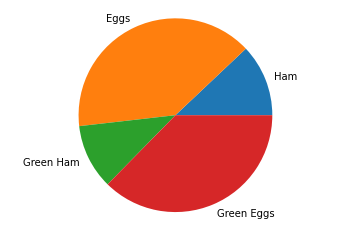
\includegraphics[width=0.8\textwidth]{img/pie1.png}

To help us read our pie plot a little easier, we can have Matplotlib insert percentages on each of the slices by specifying a format for the \verb|autopct| parameter in \verb|pie()|. This parameter uses POSIX escapes, and here, we want to specify how many digits we want, along with a percent sign. We'll use the argument \verb|%1.1f%%|, which will give us at least the ones place (the \verb|%1|, a decimal point (\verb|.|), at least one decimal place (\verb|1f|), and an escaped percent sign (\verb|%%|).

\begin{lstlisting}[style=pippython]
fig1, ax1 = plt.subplots()
ax1.pie(sizes, labels = labels, autopct = '%1.1f%%')
ax1.axis('equal')
plt.show()
\end{lstlisting}

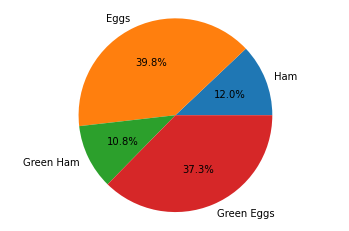
\includegraphics[width=0.8\textwidth]{img/pie2.png}

Pie plots are great for a quick comparison, but they're not very useful outside of just exploring data. Why don't we look at a histogram instead. Histograms provide more information on the distribution of the data, which is a very useful feature to statisticians.\par
Let's consider the \verb|skaters| dataset once again. What does the \verb|assists| distribution look like compared to the \verb|goals| distribution? We could run a statistical test to compare distributions, but we can also use our eyeballs to see what the data look like. Histograms bin data, then count frequencies within that bin and display that as a bar.\par
Let's start by pulling the \verb|skaters| dataset in. It is provided below for your convenience.\par
\begin{lstlisting}[style=pippython]
skaters = pd.read_pickle("https://github.com/pythonforscientists/data/blob/main/skaters.pkl?raw=true")
\end{lstlisting}
Like when we generated pie plots, we will need to generate subplots, but instead of the \verb|pie()| method on the \verb|Axes| object, we will use the \verb|hist()| method. Let's make our subplots, then making our histograms for the \verb|goals| and \verb|assists| columns.\par
\begin{lstlisting}[style=pippython]
fig1, ax1 = plt.subplots()
ax1.set_title("Goals")
ax1.hist(skaters["goals"])
fig2, ax2 = plt.subplots()
ax2.set_title("Assists")
ax2.hist(skaters["assists"])
\end{lstlisting}

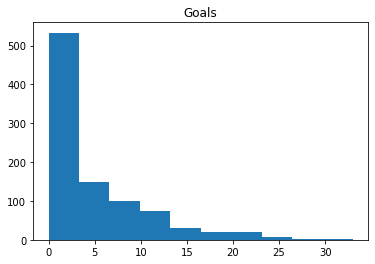
\includegraphics[width = 0.8\textwidth]{img/hist1.png}

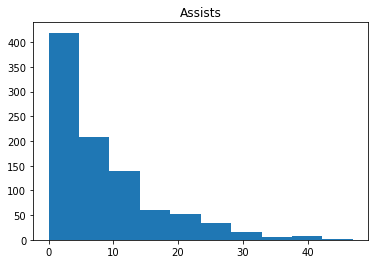
\includegraphics[width = 0.8\textwidth]{img/hist2.png}

We also threw in another method on \verb|ax1| and \verb|ax2| in this code chunk: \verb|set_title()|, which predictably, sets a title for the plot. It takes a single string argument.

This gives us some idea of what our data looks like, but what if we could view our two plots side-by-side? We can do so by specifying four parameters. The first two parameters are the shape that we want in rows, then columns. We want one row and two columns, so we'll specify the first two arguments to be \verb|1| and \verb|2|. the parameter \verb|sharey| to be \verb|True| when we create our subplot. In this case, we only want one subplot, since both of our histograms will be displayed by \verb|ax1|. We will also specify that we want to crunch the plots together by specifying the \verb|tight_layout| parameter to be \verb|True|.\par
Now, we can specify the subplot at position \verb|0| to be one of our histograms and the subplot at position \verb|1| to be the other histogram.
\begin{lstlisting}[style=pippython]
fig1, ax1 = plt.subplots(1, 2, sharey = True, tight_layout = True)
ax1[0].set_title("Goals")
ax1[0].hist(skaters["goals"])
ax1[1].set_title("Assists")
ax1[1].hist(skaters["assists"])
\end{lstlisting}

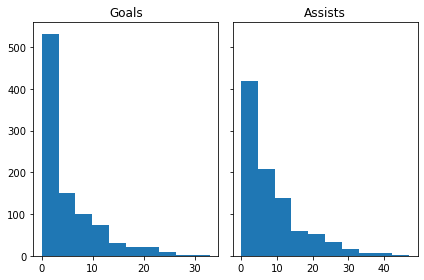
\includegraphics[width = 0.8\textwidth]{img/hist3.png}

We can also specify the number of bins that we want to use by specifying the \verb|bins| argument in the \verb|hist()| method. \verb|bins| takes an integer value.\footnote{In the below plot, we'll only set bins for the Assists plot for the sake of demonstration.}\par
\begin{lstlisting}[style=pippython]
fig1, ax1 = plt.subplots(1, 2, sharey = True, tight_layout = True)
ax1[0].set_title("Goals")
ax1[0].hist(skaters["goals"])
ax1[1].set_title("Assists")
ax1[1].hist(skaters["assists"], bins = 10)
\end{lstlisting}

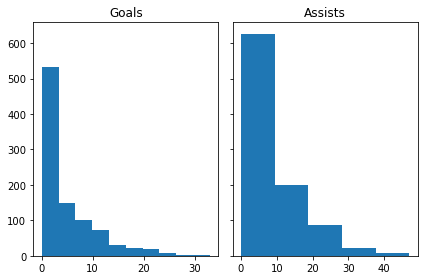
\includegraphics[width = 0.8\textwidth]{img/hist4.png}

Histograms are great for getting an idea of the shape of our distribution, but if we want to look at the data compared to the normal distribution, a better plot is a normal Q-Q plot. The normal Q-Q plot is a scatterplot created by plotting sample quantiles against theoretical quantiles from the normal distribution. If the sample quantile points are also normal, the line formed will be roughly straight, but if the sample quantile points are not normal, the line formed will not be straight and may have bends, curves, tails, and other abnormalities.\par
In Python, we'll use a combination of tools from the \verb|statsmodels| library and the \verb|matplotlib| library. Let's consider the \verb|helmets| data from earlier in this chapter. As a convenience, the data import line is provided here.\par
\begin{lstlisting}[style=pippython]
helmets = pd.read_csv("https://github.com/pythonforscientists/data/raw/main/helmets.csv")
\end{lstlisting}
Let's look at the histograms for each helmet.\par
\begin{lstlisting}[style=pippython]
fig1, ax1 = plt.subplots(1, 2, sharey = True, tight_layout = True)
ax1[0].set_title("Helmet 1")
ax1[0].hist(helmets["helmet1"])
ax1[1].set_title("Helmet 2")
ax1[1].hist(helmets["helmet2"])
\end{lstlisting}

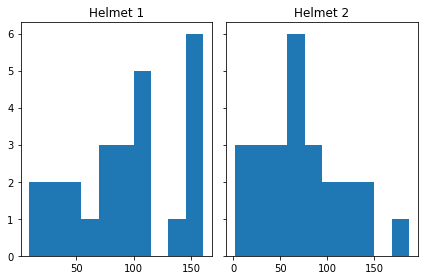
\includegraphics[width = 0.8\textwidth]{img/hist5.png}

Given these histograms, we want some more information to tell us whether either helmet is roughly normal. To do this, we can generate a normal Q-Q plot for each helmet. Let's start by importing the \verb|api| class from \verb|statsmodels|, as well as \verb|pyplot| from \verb|matplotlib| aliased as \verb|plt|.
\begin{lstlisting}[style=pippython]
import statsmodels.api
import matplotlib.pyplot as plt
\end{lstlisting}
Then, we can use the \verb|qqplot()| method from the \verb|api| class inside of \verb|statsmodels|. Then, we'll show the plot that \verb|qqplot()| made using Matplotlib's \verb|show()| method.\par
Because we have a non-zero mean, it makes sense for us to use a standardized line instead of a 45-degree line. The standardized line is created by scaling the expected order statistics by the standard deviation of the sample and having the mean added to them. If know your data are centered at zero, then you can also use \verb|'45'| instead of \verb|'s'|.\footnote{If you create normal Q-Q plots in R, the default is to create a standardized line.}
\begin{lstlisting}[style=pippython]
helmet1norm = statsmodels.api.qqplot(helmets["helmet1"], line = 's')
plt.show()
helmet2norm = statsmodels.api.qqplot(helmets["helmet2"], line = 's')
plt.show()
\end{lstlisting}

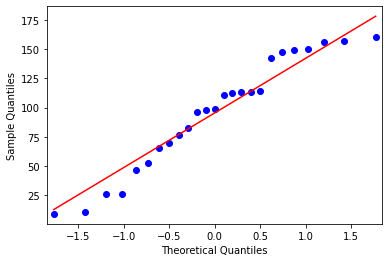
\includegraphics[width = 0.8\textwidth]{img/hist6.png}

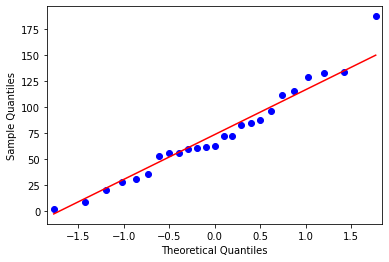
\includegraphics[width = 0.8\textwidth]{img/hist7.png}

But what if our data are not normal? Let's consider the \verb|assists| variable from the \verb|skaters| dataset. The histogram looks like the following.

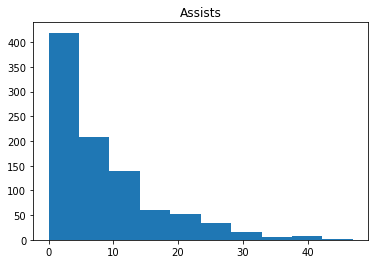
\includegraphics[width = 0.8\textwidth]{img/hist2.png}

When we create our normal Q-Q plot, it severely twists away from the standardized line.\par
\begin{lstlisting}[style=pippython]
assistsnorm = statsmodels.api.qqplot(skaters["assists"], line = 's')
plt.show()
\end{lstlisting}

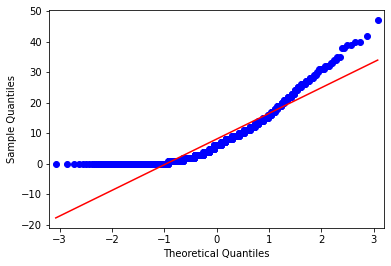
\includegraphics[width = 0.8\textwidth]{img/hist8.png}

\subsubsection*{Exercise Questions}
These exercise questions cover chapter 10.7.

No exercise questions exist for this section yet.